\documentclass[11pt]{beamer}
\usetheme{Singapore}

\usepackage[utf8]{inputenc}
\usepackage[T1]{fontenc}
\usepackage{soul}
\usepackage{graphicx}


\graphicspath{{../Figures/}}

\def\et{{\it et al.}}


\author{Cody Glickman and Michael Strong \\ NLM 2018}

\title{Enrichment of Bacterial Virulence Factors in Bacteriophages}

%\subtitle{}
%\logo{}

\date{ 
\includegraphics[height=2cm, width=2cm]{lablogo.png} \\ June, 2018}
%\subject{}
\setbeamercovered{transparent}
\setbeamertemplate{navigation symbols}{}
\setbeamertemplate{theorems}[numbered]

\begin{document}
	\maketitle

	%--------------------------------------------------------------------------------------

	
\section{Introduction}
\subsection{}

	\begin{frame}{Virulence}
		\begin{block}{Virulence Defined}
		The capacity of a microorganism to proliferate despite host defenses
		\end{block}
		
		\begin{block}{Influences on Virulence}
		\begin{itemize}
		\item Number of microorganisms
		\item \alert{Composition of the mobile genetic reservoir}
		\item Location of niche
		\item Host immune capabilities
		\end{itemize}
		\end{block}
	
	\end{frame}
	%--------------------------------------------------------------------------------------

	\begin{frame}{Bacterial Virulence Factors Increase Pathogenesis}
	\begin{columns}
	\column{0.65\textwidth}
	\begin{block}{Examples of Virulence Factors}
		\begin{itemize}
		\item Increased fitness for nutrients
		\item Host immunity resistance
		\item Toxin secretion
		\end{itemize}
	\end{block} 
	
	\begin{block}{Diseases from Virulence Factors}
	Cholera, dysentery, botulism, and food poisoning
	\end{block}
	

	\column{0.4\textwidth}
	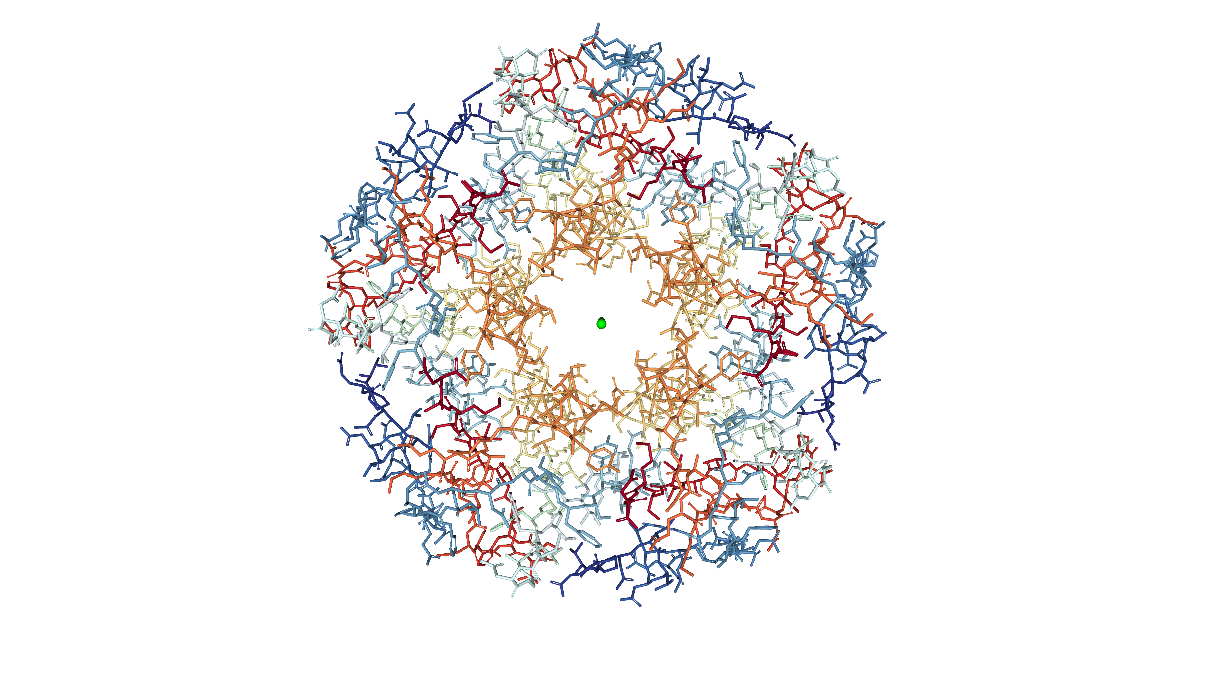
\includegraphics[height=3cm, width=5cm]{cholera.png}

	\vspace{-0.3cm}
	\hspace{0.5cm}	
	\tiny{PDB Structure of Cholera Toxin}
	\end{columns}
	
	\end{frame}
	
	%--------------------------------------------------------------------------------------
	
	\begin{frame}{Bacteriophages as a Genetic Reservoir \\ of Virulence Factors Genes}
	\begin{columns}
	\column{0.5\textwidth}
	\begin{block}{Bacteriophages (Phages)}
	DNA viruses that infect bacteria
	\end{block}
	
	
	\begin{block}{Phages and Pathology}
	Virulence Factors that cause cholera, dysentery, botulism, and food poisoning are carried on phage elements.
	\end{block}
	
	\column{0.5\textwidth}
	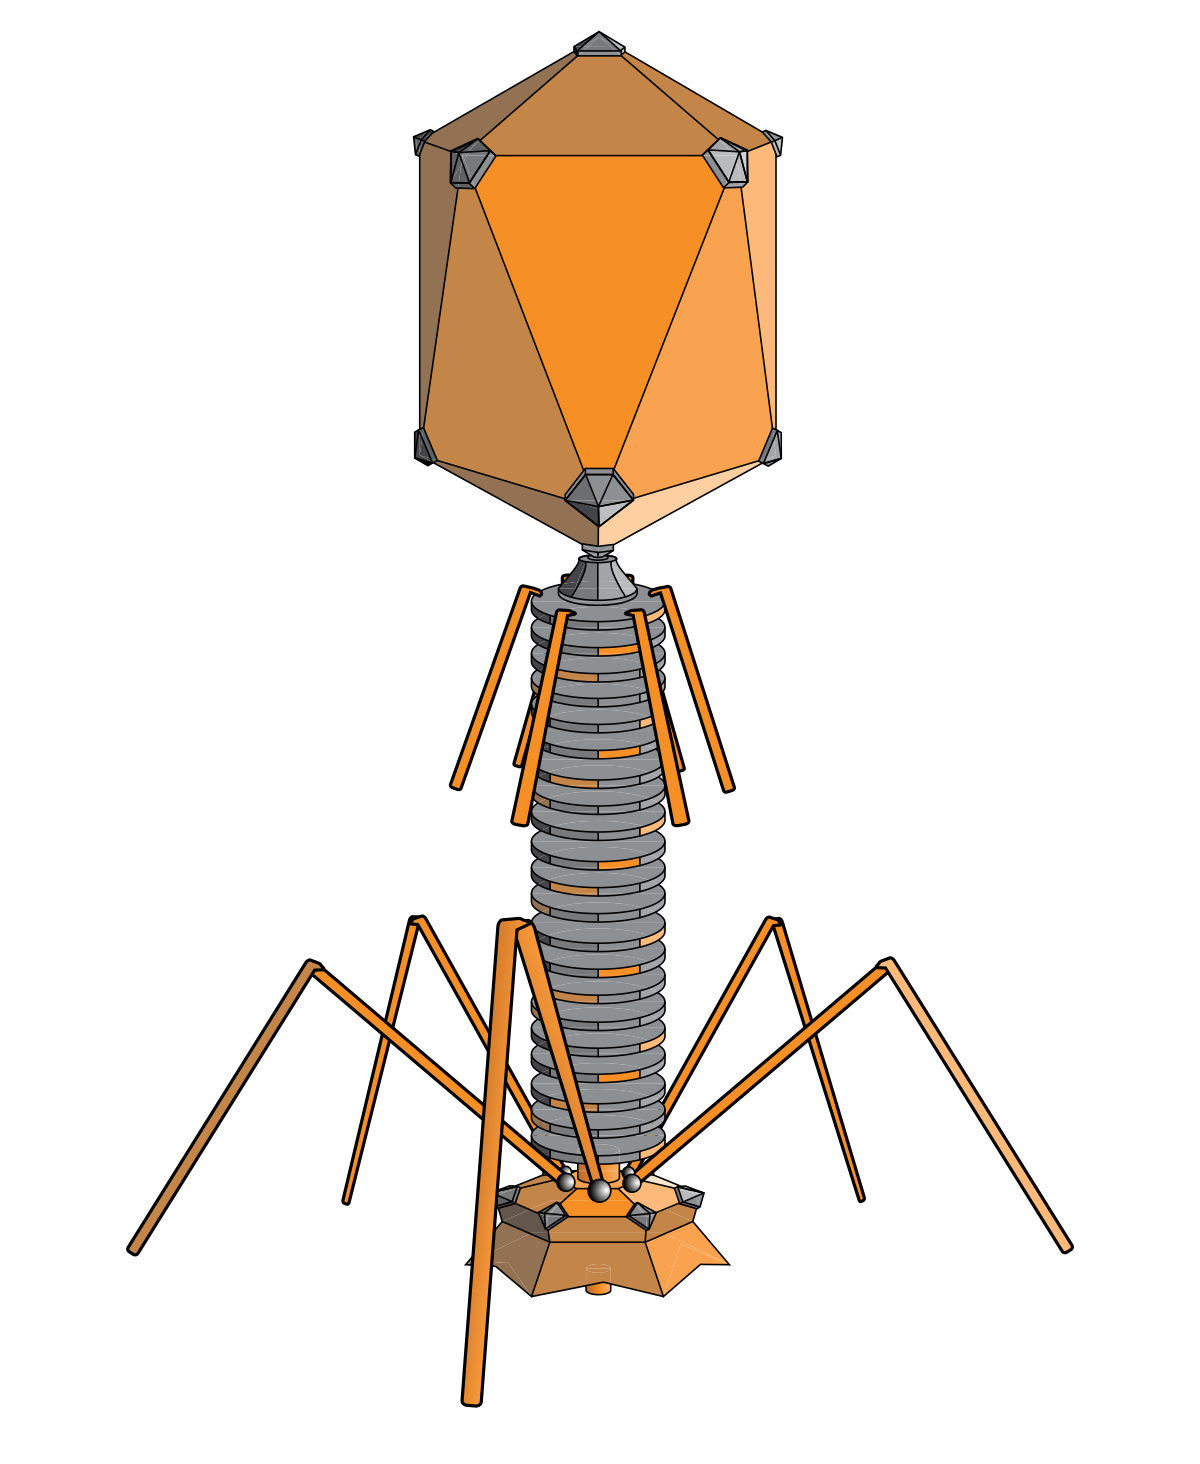
\includegraphics[height=5.5cm, width=5cm]{phage.png} \\
	\hspace{0.5cm}	
	\tiny{Novick, Richard, Plasmid (2003)}
	\end{columns}
	
	\begin{block}{Objective}
	Characterize the abundance of bacterial virulence factors in phages
	\end{block}
	
	\end{frame}

	
\section{Establishing Baseline Virulence Factor Abundance}
\subsection{}


	%-----------------------------------------	
	\begin{frame}{Data}
	\begin{columns}
	\column{0.5\textwidth}
	\begin{block}{Virulence Protein Databases}
		\begin{itemize}
			\item VFDB \\ \tiny{Chen, Lihong, et al. Nucleic Acids Research (2005)}
			\item \large{PatricVF} \\ \tiny{Wattam, AR, et al. Nucleic Acids Research (2017)}
		\end{itemize}
	\end{block}
	\begin{block}{Virulence HMMs}
	\begin{itemize}
		\item pFam \\ \tiny{Bateman, Alex, et al. Nucleic Acids Research (2004)}
		\item \large{pVOG} \\ \tiny{Grazziotin, AL, et al. Nucleic Acids Research (2016)}
	\end{itemize}
	\end{block}
	
	
	\column{0.5\textwidth}
	\begin{block}{Phage Protein Database}
	
\includegraphics[height=3cm, width=3cm]{uniprot.png}
	\end{block}
	\end{columns}
	\end{frame}

	%-----------------------------------------	
	\begin{frame}{Methods}
	\begin{columns}
	\column{0.7\textwidth}
	\begin{block}{Sequence Annotation Methods}
	BLAST vs \alert{HMM}
	\end{block}
	
	\begin{block}{Normalizing By Gene Count}
	Hit Percentage = $P$ \\
	Hit Count = $HC$ \\
	Gene Count = $GC$ \\
	\vspace{0.3cm}
	\hspace{1.5cm}	
	$P = {HC}/{GC}$
	\end{block}
	
	\begin{block}{Filtering By Phage Abundance}
	\alert{Streptococcus} phage: \\
	Genera abundance greater than 30
	\end{block}
	
	
	
	\column{0.2\textwidth}
	\hspace{-2cm}
	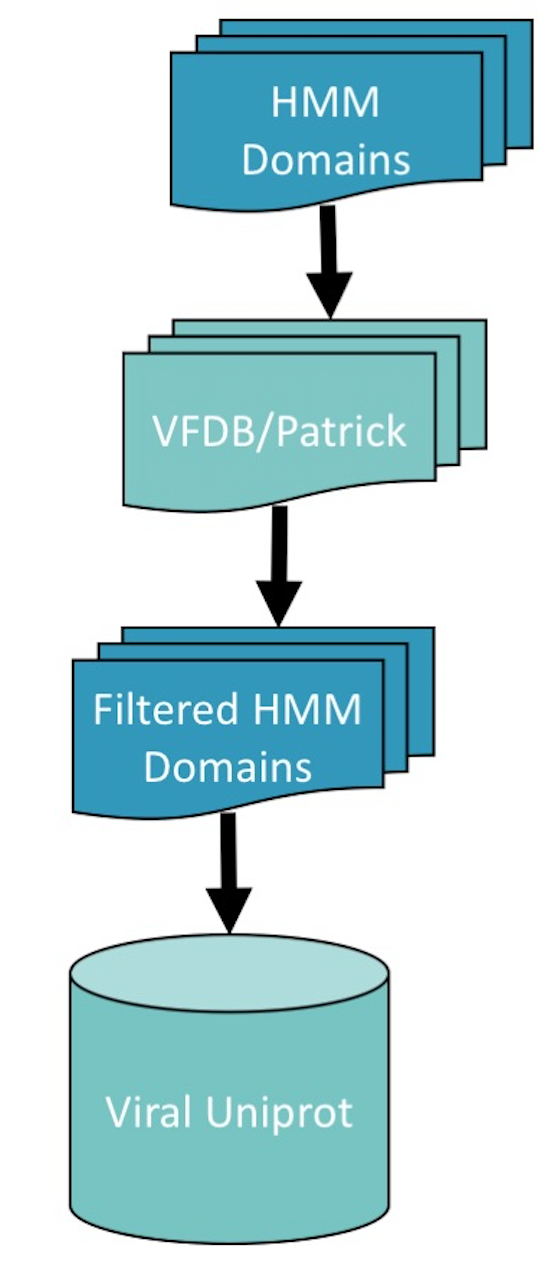
\includegraphics[height=6cm, width=3cm]{Pipeline.png}

	\end{columns}
	\end{frame}
	
	
	%-----------------------------------------	
	\begin{frame}{HMM Hit Distribution}
	\begin{columns}
	\column{0.6\textwidth}
	% Need to place figure
	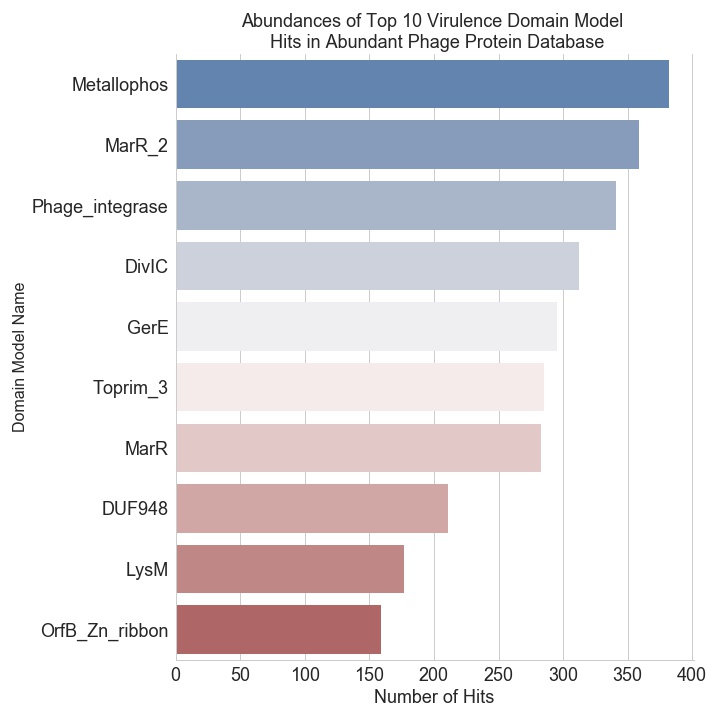
\includegraphics[height=6cm, width=6cm]{Abundant_Phages_HMM_ID.jpg}
	\column{0.5\textwidth}
	\begin{block}{MarR}
	Domain involved in antibiotic resistance
	\end{block}
	\begin{block}{DivIC}
	Part of sporulation process
	\end{block}
	\begin{block}{LysM}
	General peptidoglycan function
	\end{block}
	\end{columns}
	\end{frame}
	
	%-----------------------------------------	
	\begin{frame}{Distribution of Hit Percentage in All Phages}
	\centering
	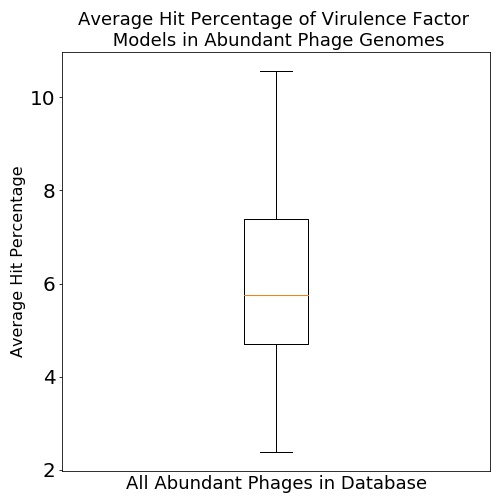
\includegraphics[height=7cm, width=7cm]{Abundant_Phages_Percentage.jpg}
	
	\end{frame}
	
	%-----------------------------------------	
	\begin{frame}{Abundant Phage Distributions by Genera Name}
	\centering
	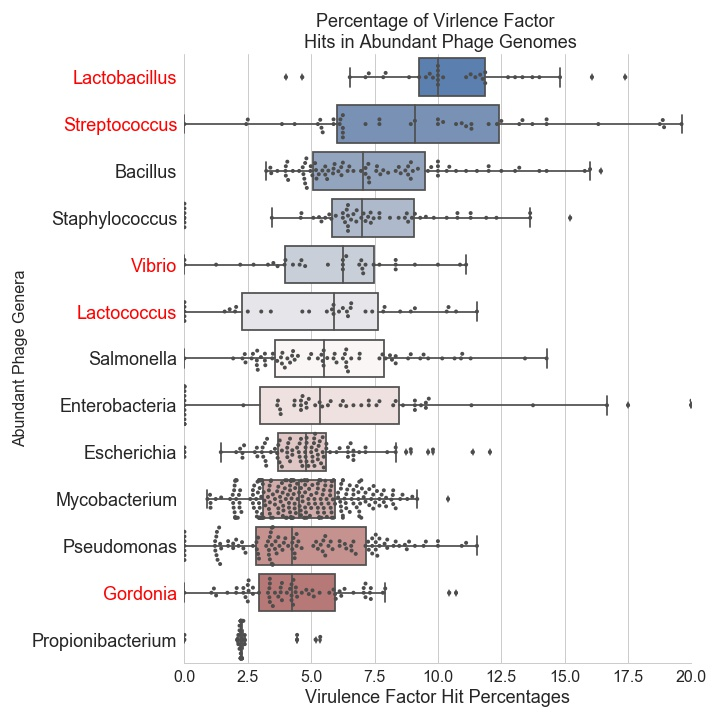
\includegraphics[height=7cm, width=8cm]{Top_Phages_Plots.jpg}
	
	\end{frame}
	
	

\section{Virulence Factors in Clinical Viral Metagenome}
\subsection{}

	%-----------------------------------------	
	\begin{frame}{Clinical Data and Methodology}
	\begin{block}{Clinical Data Sources}
	\begin{itemize}
	\item \large{Virome from Cystic Fibrosis Patients} \\ \tiny{PRJNA39545}
	\item \large{Virome from Clostridium difficile Patients} \\ \tiny{PRJEB22784}
	\end{itemize}
	\end{block}
	\begin{block}{Clinical Data Pipeline}
	\centering
	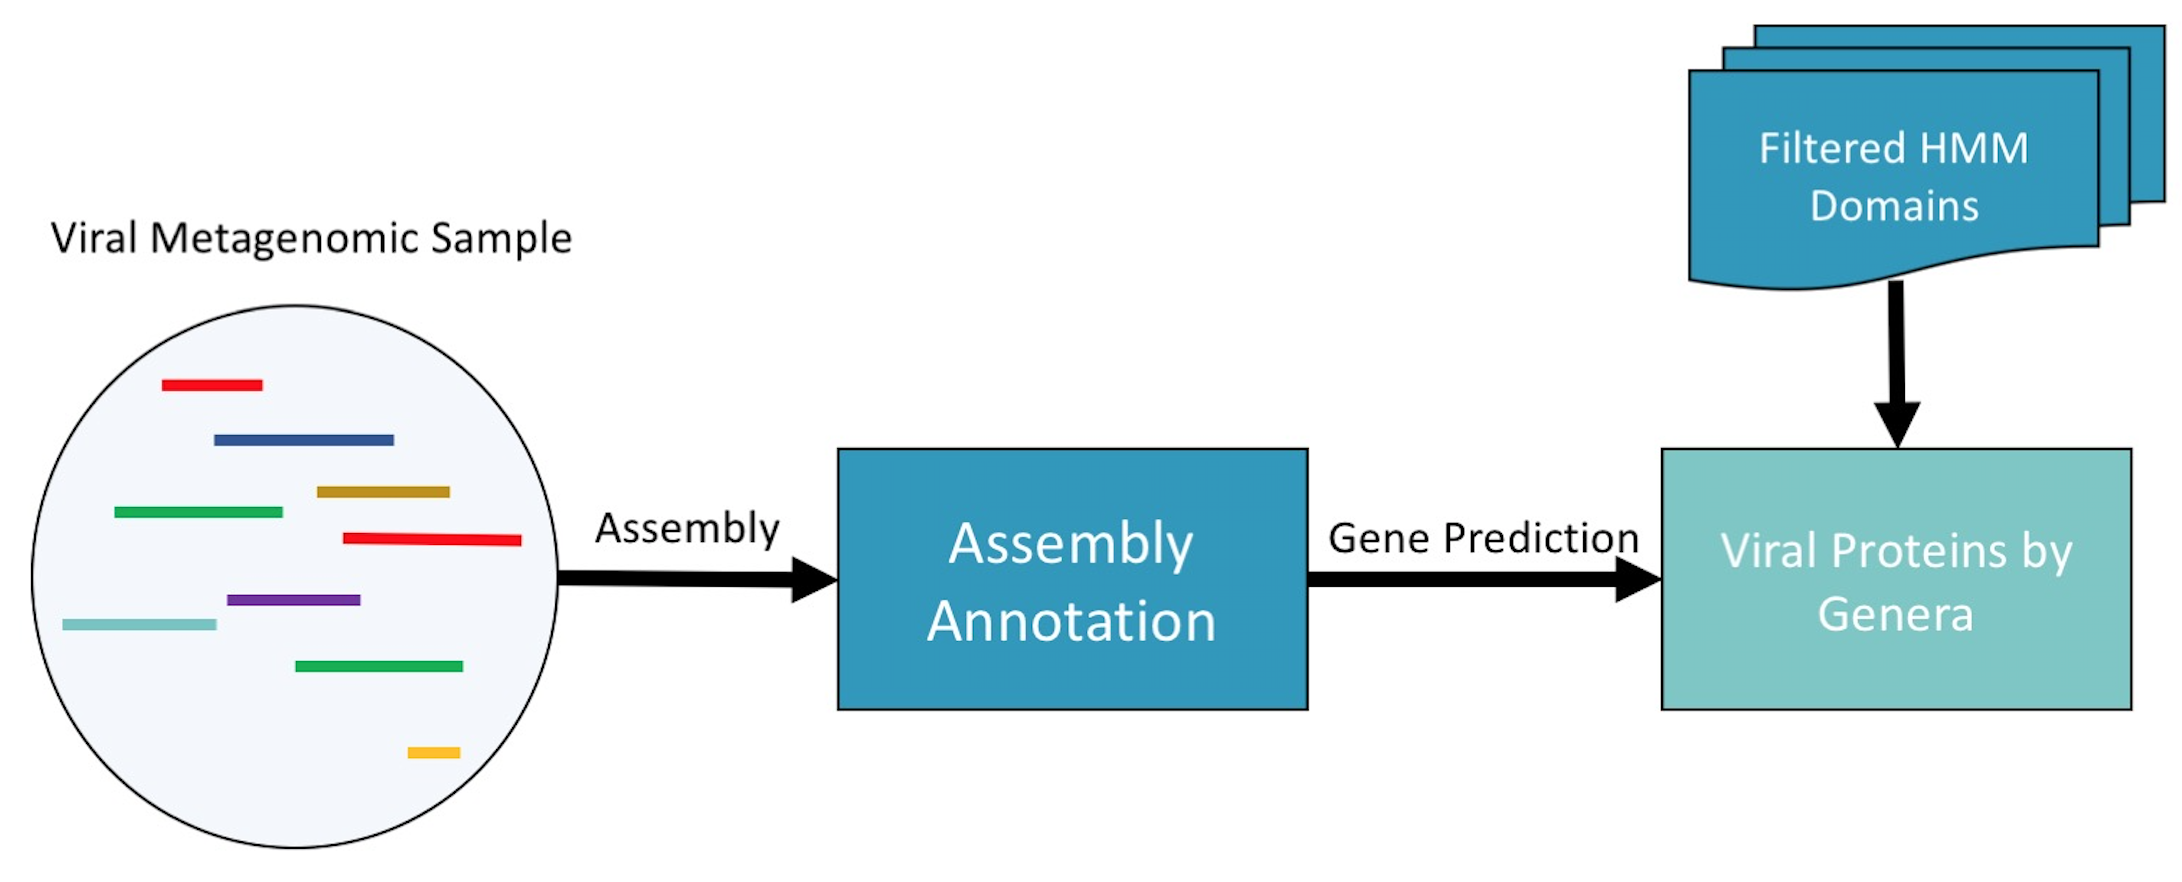
\includegraphics[height=5cm, width=10cm]{Clinical_Pipeline.png}
	\end{block}
	\end{frame}
	
	%-----------------------------------------	
	\begin{frame}{Cystic Fibrosis Virome Results}
	\begin{columns}
	\column{0.4\textwidth}
	\hspace{2cm}
	\begin{block}{Abundant Annotated Genera (>20 Contigs)}
	\begin{itemize}
	\item \alert{Streptococcus Phage}
	\item Enterobacteria Phage
	\item Staphylococcus Phage
  \end{itemize}
  \end{block}
  
  \begin{block}{Nonparametric Testing}
  $H_o$: Samples == Baseline \\
  \vspace{0.2cm}
  $p =$ 0.487
  \end{block}
	
	
	
	
	\column{0.7\textwidth}
	\centering
	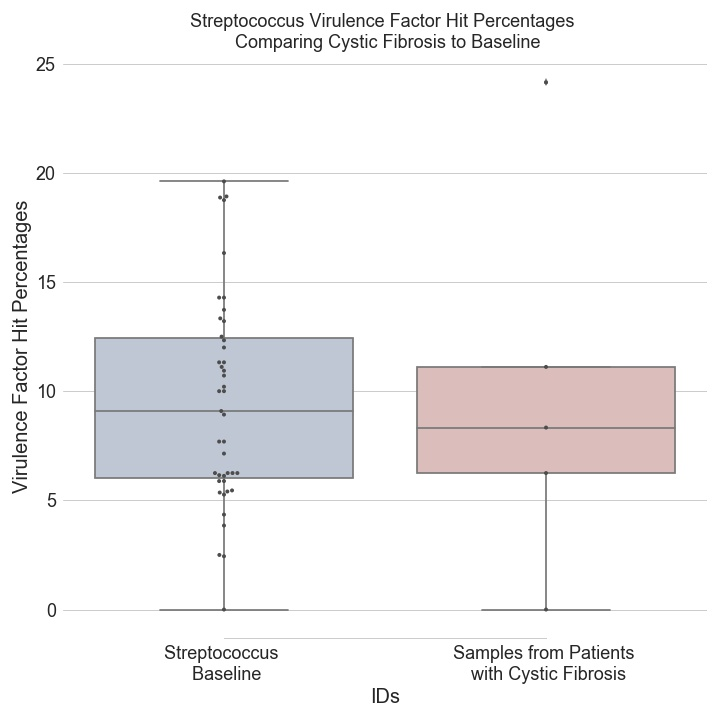
\includegraphics[height=7cm, width=6cm]{CF_Comparison.jpg}
	
	
	\end{columns}
	
	\end{frame}
	%-----------------------------------------
  \begin{frame}{Clostridium difficile Virome Results}
  \begin{columns}
	\column{0.4\textwidth}
	\hspace{2cm}
	\begin{block}{Abundant Annotated Genera (>20 Contigs)}
	\begin{itemize}
	\item \alert{Salmonella Phage}
	\item Pseudomonas Phage
	\item Escherichia Phage
	\item Enterobacteria Phage
  \end{itemize}
  \end{block}
  
  \begin{block}{Unequal Variance \\ Parametric Testing}
  $H_o$: Samples == Baseline \\
  \vspace{0.2cm}
  $p =$ 0.09
  \end{block}
  
  \column{0.7\textwidth}
	\centering
	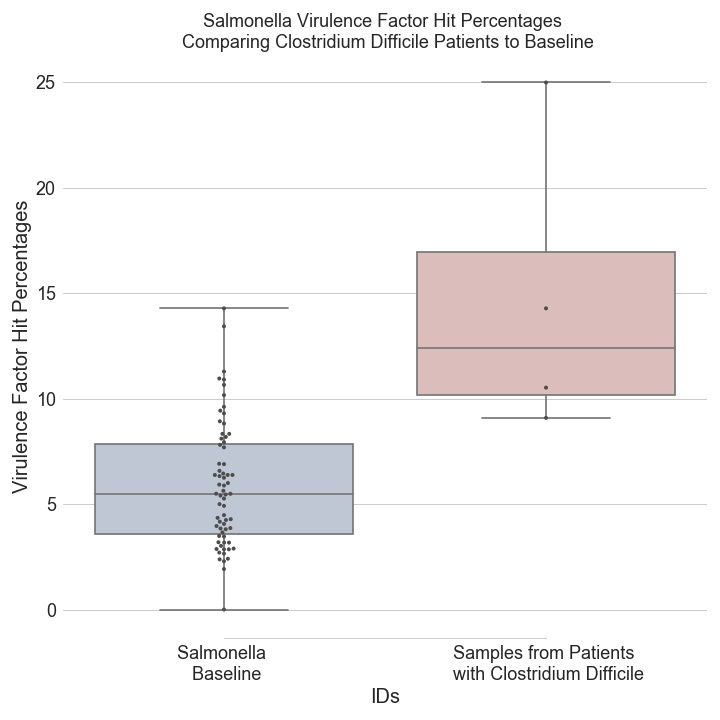
\includegraphics[height=7cm, width=6cm]{CDif_Comparison.jpg}
	
	\end{columns}
	
	\end{frame}
	
\section{}

	%-----------------------------------------	
	\begin{frame}{Concluding Remarks}
	\begin{columns}
	\column{0.6\textwidth}
	\begin{block}{Virulence Factor Abundance}
	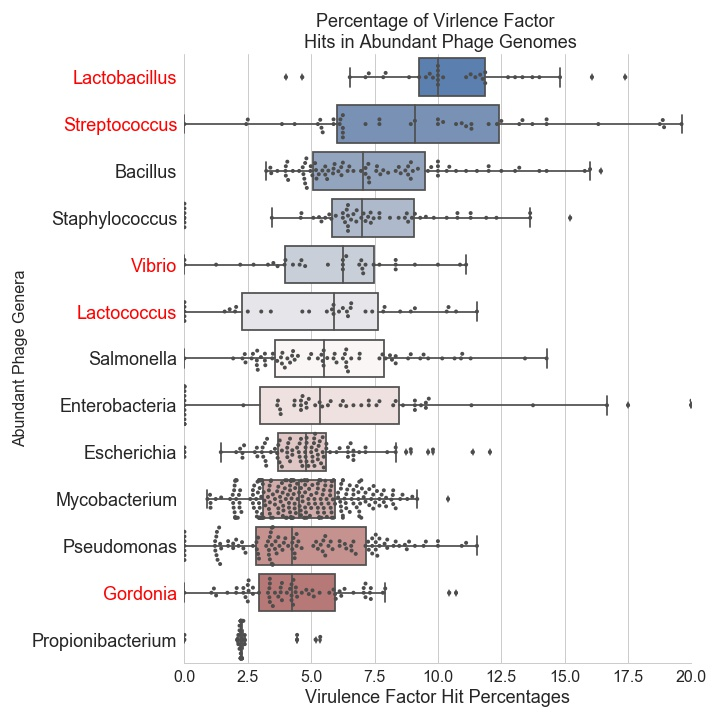
\includegraphics[height=7cm, width=6cm]{Top_Phages_Plots.jpg}
	\end{block}
	\column{0.5\textwidth}
	\begin{block}{Clinical Virulence Distribution}
	Trending enrichment of virulence hits in Salmonella phages in patients with Clostridium difficile infections
	\end{block}
	\begin{block}{Research in Progress}
	Application to Non-Tuberculosis Mycobacterium infections in Cystic Fibrosis patients
	\end{block}
	
	\end{columns}
	
	\end{frame}
	
	
	
	%-----------------------------------------	
	\begin{frame}{Acknowledgements}
	\centering
	{
\includegraphics[height=5cm, width=11cm]{Acknowledgements.png} }
	\end{frame}
	
	%-----------------------------------------	
	\begin{frame}{Questions?}
	\center
	Cody Glickman \\ 
\includegraphics[height=2cm, width=2cm]{lablogo.png} \\ cody.glickman@ucdenver.edu \\ \alert{www.github.com/glickmac} \\ www.codyglickman.com
	\end{frame}


\end{document}